\chapter{Full Channel, Narrowband Analysis}
\label{chap:full_narrow}

The analysis now expands from the LOS model to a more comprehensive full-channel model. This section considers the impact of multiray components generated by reflections off the buildings lining. The analysis remains within the narrowband regime, where the channel's response can be characterized by a single complex coefficient, but this coefficient now incorporates the vector sum of all significant propagation rays, not just the direct one.


In a realistic urban environment, the signal transmitted from TX to RX does not travel along a single ray. Instead, it propagates along multiple rays due to reflections from surrounding objects, in this case, the building facades. Each of these rays is an MPC. The total received signal is the vector sum of all these MPCs. The narrowband channel transfer function, previously represented by a single complex gain $\alpha_1$ for the LOS ray, is now the sum of the complex gains of all MPCs:
\begin{equation}
	h_{NB} = \sum_{n=1}^{N} \alpha_n
\end{equation}
where $N$ is the total number of MPCs, including the LOS ray and all reflected rays. Each complex gain $\alpha_n$ is a function of the ray's length, the reflection coefficients of the surfaces it interacts with, and the propagation delay.

The primary tool for identifying these rays and calculating their geometry is the \textbf{image method}. For each reflecting surface, an image of the transmitter is created. A straight line from this image to the receiver identifies the ray of the reflected wave, as shown in Figure \ref{fig:image_method_single}. This method can be extended recursively to find rays with multiple reflections.

\begin{figure}[h!]
	\centering
	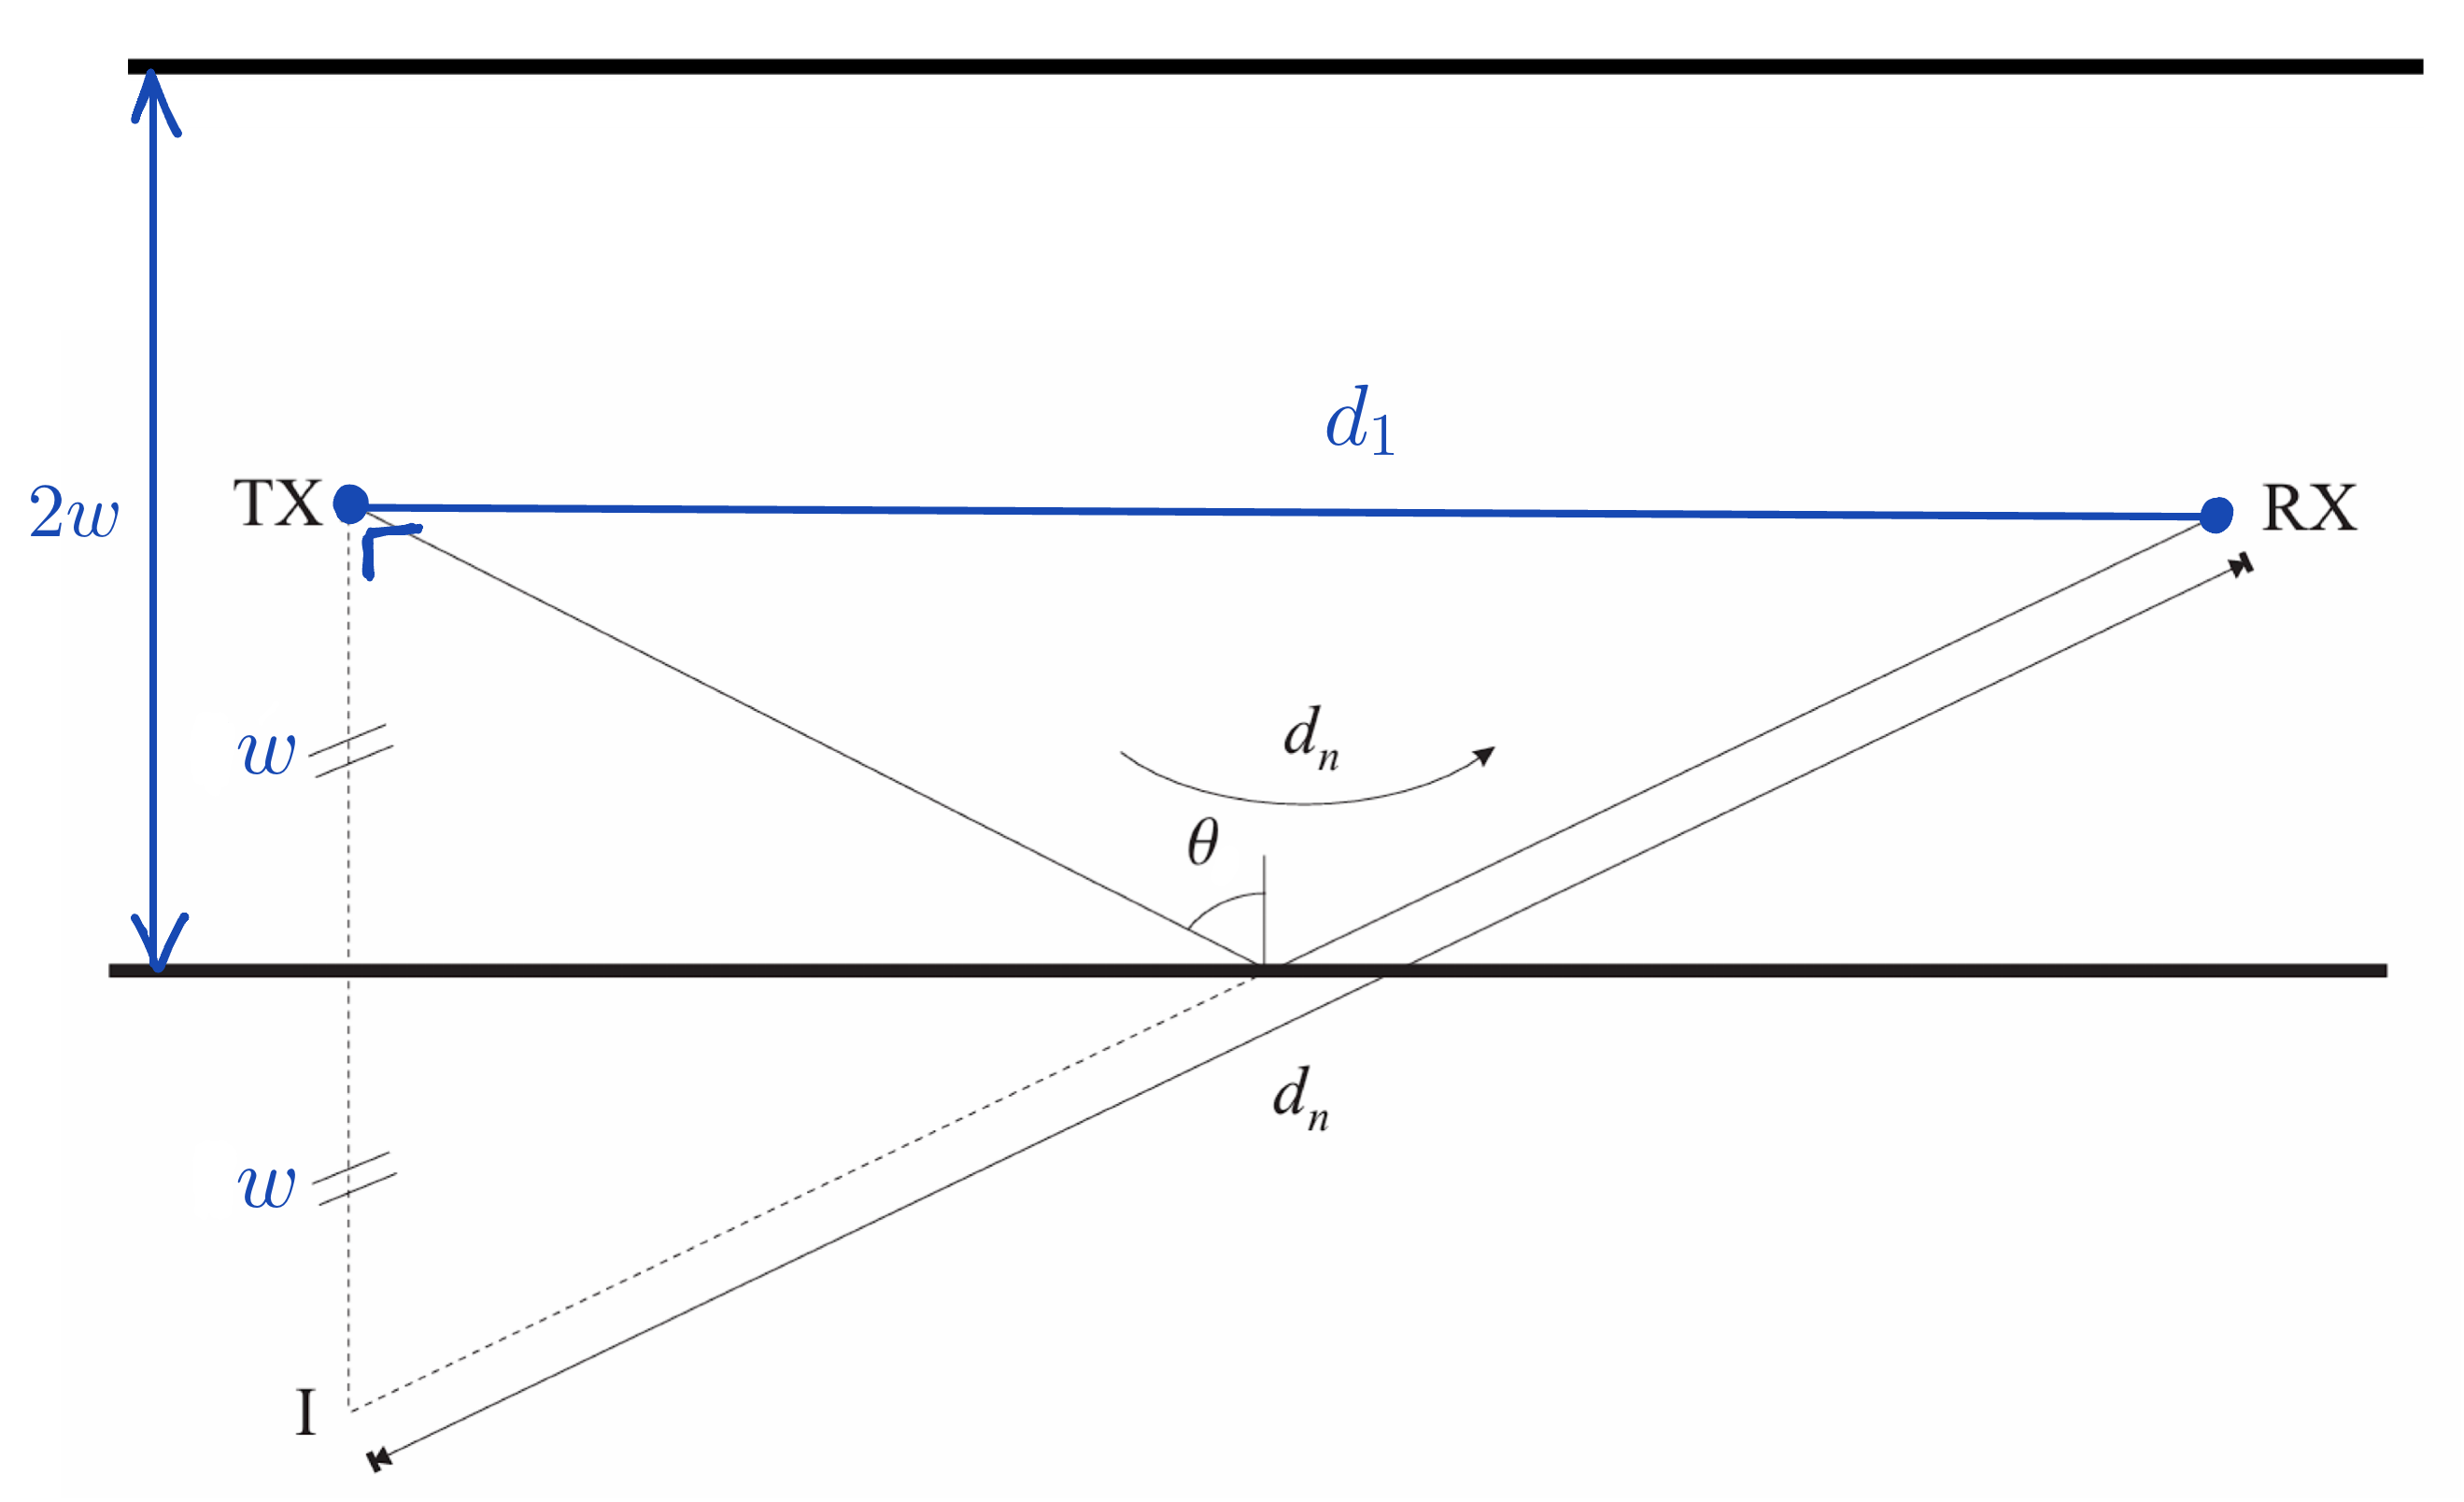
\includegraphics[width=0.7\linewidth]{content/4-images/image-method.png}
	\caption{The image method for a single reflection. The ray of the reflected ray from TX to RX is found by drawing a straight line from the image transmitter I to RX.}
	\label{fig:image_method_single}
\end{figure}


\section{Multiray Component Geometry}
To find the paths of all significant rays, we use the image method. The scenario is a urban street of width $2w = 20$ m. The transmitter TX and receiver RX are placed symmetrically in the center of the street, separated by a distance $d$. The building walls are represented by two parallel lines at $y = w$ and $y = -w$.

\subsubsection{LOS ray}
The LOS ray is the direct, unobstructed path between the transmitter and receiver. It is considered as the first path component, meaning $n=1$.
\begin{itemize}
	\item \textbf{Path Length: $d_1 = d$} The
	\item \textbf{Propagation Delay:}
	\begin{equation}
		\tau_{1} = \frac{d}{c}
	\end{equation}
\end{itemize}

\subsubsection{Single Reflection rays}
There are two distinct paths involving one reflection, one from the top wall and one from the bottom wall. Using the image method, we create a virtual source $I_1$ by reflecting the TX across the wall. The path length is the straight-line distance from $I_1$ to the RX.
\begin{itemize}
	\item \textbf{Path Length:} The geometry forms a right triangle with legs and $d$ and $2w$ (the vertical distance between the image and the RX).
	\begin{equation}
		d_{n} = \sqrt{d^2 + (2w)^2}
	\end{equation}
	\item \textbf{Propagation Delay:}
	\begin{equation}
		\tau_{n} = \frac{\sqrt{d^2 + (2w)^2}}{c}
	\end{equation}
	\item \textbf{Angle of Incidence:} The angle of incidence with the wall is given by:
	\begin{equation}
		\sin(\theta_{n}) = \frac{d}{d_{n}}
	\end{equation}
\end{itemize}

\subsubsection{Double Reflection rays}
There are two paths involving two reflections (e.g. Wall 1 $\rightarrow$ Wall 2 $\rightarrow$ RX). To find the path length, we create a second-order image $I_2$, by reflecting the first-order image $I_1$ across the opposite wall.
\begin{itemize}
	\item \textbf{Path Length:} The vertical separation between the second-order image $I_2$ and the RX is now $4w$.
	\begin{equation}
		d_{n} = \sqrt{d^2 + (4w)^2}
	\end{equation}
	\item \textbf{Propagation Delay:}
	\begin{equation}
		\tau_{n} = \frac{\sqrt{d^2 + (4w)^2}}{c}
	\end{equation}
	 \item \textbf{Angle of Incidence:} The angle of incidence is the same for both reflections and is given by:
	\begin{equation}
		\cos(\theta_{n}) = \frac{d}{d_{n}} = \frac{d}{\sqrt{d^2 + (4w)^2}}
	\end{equation}
\end{itemize}


\subsubsection{K-th Order Reflection Rays (Recursive Approach)}
While closed-form expressions can be derived for this simple geometry, a more robust and general method is to define the process recursively, as implemented in the simulation. To find all paths with up to $K$ reflections, the algorithm extends the image method by systematically generating and validating potential ray paths.

This process is implemented using the recursive function \texttt{findReflectedRaysRecursive}, which builds a tree of image sources as illustrated in Figure \ref{fig:image_tree}. The function starts with the real transmitter (the 0-order source) and the desired number of reflections. In each recursive step, it mirrors the current source across every wall in the environment using \texttt{findSymmetricAcrossLine}, creating a new set of higher-order image sources. It then calls itself for each new image, with the remaining number of reflections decremented. To avoid physically redundant paths, a source is never immediately reflected back across the same wall it was just generated from.

\begin{figure}[h!]
	\centering
	%====================================================================================
	% TIKZ PREAMBLE REQUIREMENTS
	% To compile this figure, ensure you have the following lines in your main .tex file's preamble:
	% \usepackage{tikz}
	% \usetikzlibrary{arrows.meta, positioning}
	% The 'positioning' library is used for the "below left/right=of" syntax.
	%====================================================================================
	\begin{tikzpicture}[
		% Set distances for manual placement
		node distance=1.5cm and 2.5cm,
		% Common style for all nodes in the diagram
		every node/.style={
			shape=rectangle,
			rounded corners,
			draw,
			align=center,
			top color=white,
			bottom color=blue!20
		},
		% Style for the connecting arrows
		arrow/.style={draw, -{Latex[length=2mm]}}
		]
		% Place nodes manually using the 'positioning' library features
		\node (root) {TX (Order 0)};
		\node (c1) [below left=of root] {$I_{W1}$ (Order 1)};
		\node (c2) [below right=of root] {$I_{W2}$ (Order 1)};
		\node (c11) [below=1.5cm of c1] {$I_{W1,W2}$ (Order 2)};
		\node (c21) [below=1.5cm of c2] {$I_{W2,W1}$ (Order 2)};
		\node (c111) [below=of c11] {$\dots$};
		\node (c211) [below=of c21] {$\dots$};
		
		% Draw the arrows and place the styled labels on them
		% The 'node' command here creates a label that inherits the 'every node' style
		\path[arrow] (root.south) -- (c1.north)
		node[midway, sloped, font=\ttfamily] {mirror(TX, W1)};
		\path[arrow] (root.south) -- (c2.north)
		node[midway, sloped, font=\ttfamily] {mirror(TX, W2)};
		
		% Draw the rest of the arrows
		\path[arrow] (c1) -- (c11);
		\path[arrow] (c2) -- (c21);
		\path[arrow] (c11) -- (c111);
		\path[arrow] (c21) -- (c211);
	\end{tikzpicture}
	\caption{Conceptual tree of image sources generated by \texttt{findReflectedRaysRecursive}. Each level corresponds to an order of reflection.}
	\label{fig:image_tree}
\end{figure}

The recursion stops when the desired reflection order is reached. At this point, the sequence of image sources defines a potential ray path. However, this path is only geometrically hypothetical. It must be validated by the \texttt{validateRayPath} function, which traces the path backward from RX to TX. The logic of this validation is detailed in the flowchart in Figure \ref{fig:validation_flowchart}.

\begin{figure}[h!]
	\centering
	%====================================================================================
	% TIKZ PREAMBLE REQUIREMENTS
	% To compile this figure, ensure you have the following lines in your main .tex file's preamble:
	% \usepackage{tikz}
	% \usetikzlibrary{arrows.meta, positioning, shapes.geometric}
	% The 'shapes.geometric' library is essential for the diamond shape.
	%====================================================================================
	\begin{tikzpicture}[
		node distance=1.3cm and 1cm,
		block/.style={rectangle, draw, fill=blue!20, text width=10em, text centered, rounded corners, minimum height=3em},
		line/.style={draw, -{Latex[length=2mm]}},
		decision/.style={diamond, draw, fill=green!20, text width=5.5em, text centered, aspect=1.5, inner sep=0pt}
		]
		% Nodes
		\node [block] (start) {Start with RX,\\ images: ($I_M \dots I_1$); walls: ($W_M \dots W_1$). Let $m=M$.};
		\node [block, below=of start] (intersect) {Cast ray from current point to $I_M$. Find intersection $R_m$ on wall $W_m$.};
		\node [decision, below=of intersect] (dec1) {$R_m$ on wall segment?};
		\node [block, below=of dec1] (obstruct) {Check segment from $R_m$ to previous point for obstructions.};
		\node [decision, below=of obstruct] (dec2) {Obstructed?};
		\node [decision, below=of dec2] (dec3) {$m=1$? (Last segment)};
		\node [block, left=of dec3, xshift=-1cm] (loop) {Decrement $m$. Set $R_m$ as new current point.};
		\node [block, right=of dec1, xshift=1cm, fill=red!30] (invalid1) {Path Invalid};
		\node [block, right=of dec2, xshift=1cm, fill=red!30] (invalid2) {Path Invalid};
		\node [block, below=of dec3, fill=green!30] (valid) {Path Valid!};
		
		% Paths
		\path [line] (start) -- (intersect);
		\path [line] (intersect) -- (dec1);
		\path [line] (dec1) -- node[anchor=east] {Yes} (obstruct);
		\path [line] (dec1) -- node[anchor=south] {No} (invalid1);
		\path [line] (obstruct) -- (dec2);
		\path [line] (dec2) -- node[anchor=south] {Yes} (invalid2);
		\path [line] (dec2) -- node[anchor=east] {No} (dec3);
		\path [line] (dec3) -- node[anchor=east] {Yes} (valid);
		\path [line] (dec3) -- node[anchor=north] {No} (loop);
		\path [line] (loop) |- (intersect);
		
	\end{tikzpicture}
	\caption{Flowchart of the backward path validation process in \texttt{validateRayPath}.}
	\label{fig:validation_flowchart}
\end{figure}

The validation process follows the sequence:
\begin{enumerate}
	\item Starting from the RX, a line is cast to the final image source ($I_M$). Its intersection with the corresponding wall segment ($W_M$) is found using \texttt{findSegmentIntersection}. If an intersection point does not exist on the finite wall segment, the path is invalid.
	\item If the reflection point is valid, the path segment from it to the RX is checked for obstructions by any other wall. If it is obstructed, the path is invalid.
	\item The process is then repeated, tracing backward from the newly found reflection point to the next image in the sequence ($I_{K-1}$) to find the next reflection point on its respective wall ($W_{K-1}$).
	\item This continues until the entire path has been traced back to the original transmitter. A path is only considered valid if every segment is unobstructed and every reflection point lies on its physical wall.
\end{enumerate}

Once $n$-th ray path is validated, the function \texttt{calculatePhysicalProperties} computes its total path length $d_n$, by summing the lengths of its segments. It also calculates the angle of incidence for each reflection to find the product of the Fresnel reflection coefficients.

For the specific symmetric  geometry of the setup, this recursive algorithm correctly identifies the paths whose lengths are given by the simplified formula:
\begin{equation}
	d_{n} = \sqrt{d^2 + (2Mw)^2}
\end{equation}
The corresponding propagation delay is:
\begin{equation}
	\tau_{n} = \frac{\sqrt{d^2 + (2Mw)^2}}{c}
\end{equation}
An the Angle of incidence is defined by:
\begin{equation}
	\cos(\theta_{n}) = \frac{d}{d_{n}} = \frac{d}{\sqrt{d^2 + (2Mw)^2}}
\end{equation}

For a simulation considering up to $M=10$ reflections, this process identifies the LOS ray plus two rays for each reflection order, resulting in a total of $N=1+2\times10=21$ valid MPCs.

\begin{figure}
	\centering
	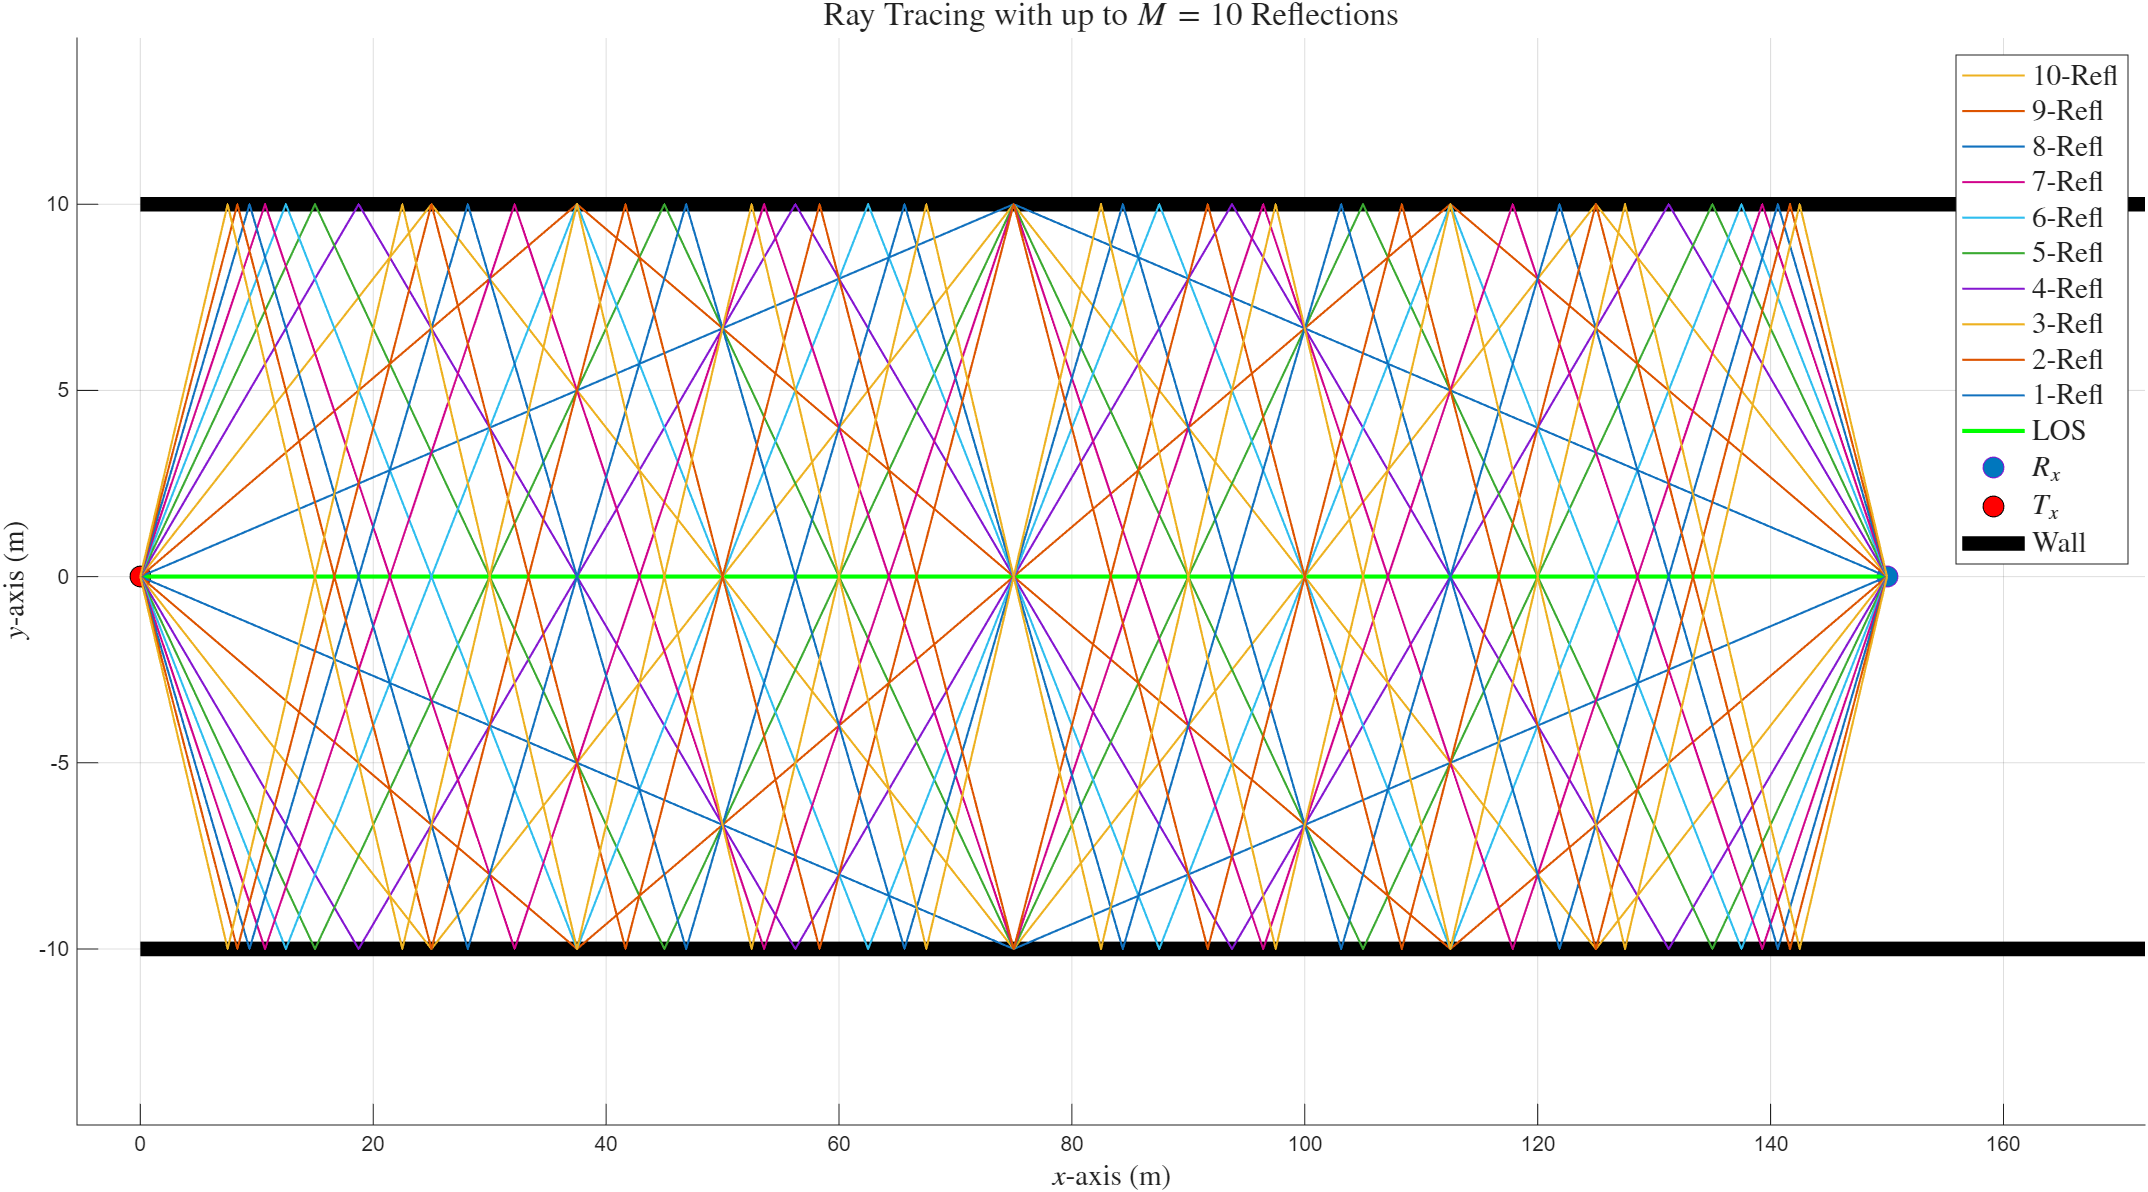
\includegraphics[width=\linewidth]{content/4-images/ray-tracing-10-reflections.png}
	\caption{Simulation of the image method ray-tracing for 10 reflections, showing the 21 valid MPCs found.}
	\label{fig:raytracing-3reflex}
\end{figure}



\section{Total Received Voltage}
The complex amplitude $\alpha_n$ for each ray $n$ must account for the path loss and any phase changes from reflections. The general form for the complex amplitude of a ray of length $d_n$ with $M$ reflections is:
\begin{equation}
	\alpha_n = \left( j \frac{\lambda Z_0}{4\pi^2 R_a d_n} e^{-j2\pi f_c \tau_n} \right) \times \prod_{m=1}^{M}(\Gamma_{\perp, m}(\theta_{n}))
\end{equation}
where $\Gamma_{\perp}$ is the reflection coefficient for perpendicular polarization for the $n$-th MPC experiencing $M$ reflections:
\begin{equation}
	\Gamma_{\perp, m}(\theta_n) = \frac{\cos\theta_n - \sqrt{\epsilon_{r, m} - \sin^2\theta_n}}{\cos\theta_n + \sqrt{\epsilon_{r, m} - \sin^2\theta_m}}
\end{equation}
with $\epsilon_{r,m} = 4$ for the buildings. The angle of incidence $\theta_n$ is specific to each reflection order.

The narrowband transfer function found in Equation \eqref{eq:narrow} is given by :
\begin{equation}
	h_{NB} = \sum_{n=1}^{N=7} \alpha_n = \alpha_{LOS} + \sum_{n=2}^{N=7} \alpha_n
\end{equation}

The total received voltage $\underline{V}_{RX}$ is then:
\begin{equation}
	\underline{V}_{RX} = \frac{h_{NB}}{2} \underline{V}_{TX}
\end{equation}



\textcolor{red}{TABLE OF VALUES FOR THE FIRST M REFLECTIONS}



\section{Received Power and Comparison with Friis Formula}

The received power is:
\begin{equation}
	P_{RX} = |h_{NB}|^2 P_{TX} = \left| \alpha_{LOS} + \sum_{n=2}^{N=7} \alpha_n \right|^2 P_{TX}
\end{equation}
This expression highlights the difference from the LOS only represented by the Friis formula:
\begin{equation}
	P_{RX, \text{Friis}} = P_{TX} G_{TX} G_{RX} \left( \frac{\lambda}{4\pi d} \right)^2 = |\alpha_{LOS}|^2 P_{TX}
\end{equation}
The Friis formula represents the power of only the first term ($n=1$) in the sum. In the full channel model, the total power depends on the vector sum of all 7 MPCs. Because the rays have different lengths $d_n$ and undergo different phase shifts ($e^{-j2\pi f_c \tau_n}$ and from reflections), the complex amplitudes $\alpha_n$ add up coherently.

\begin{figure}[H]
	\centering
	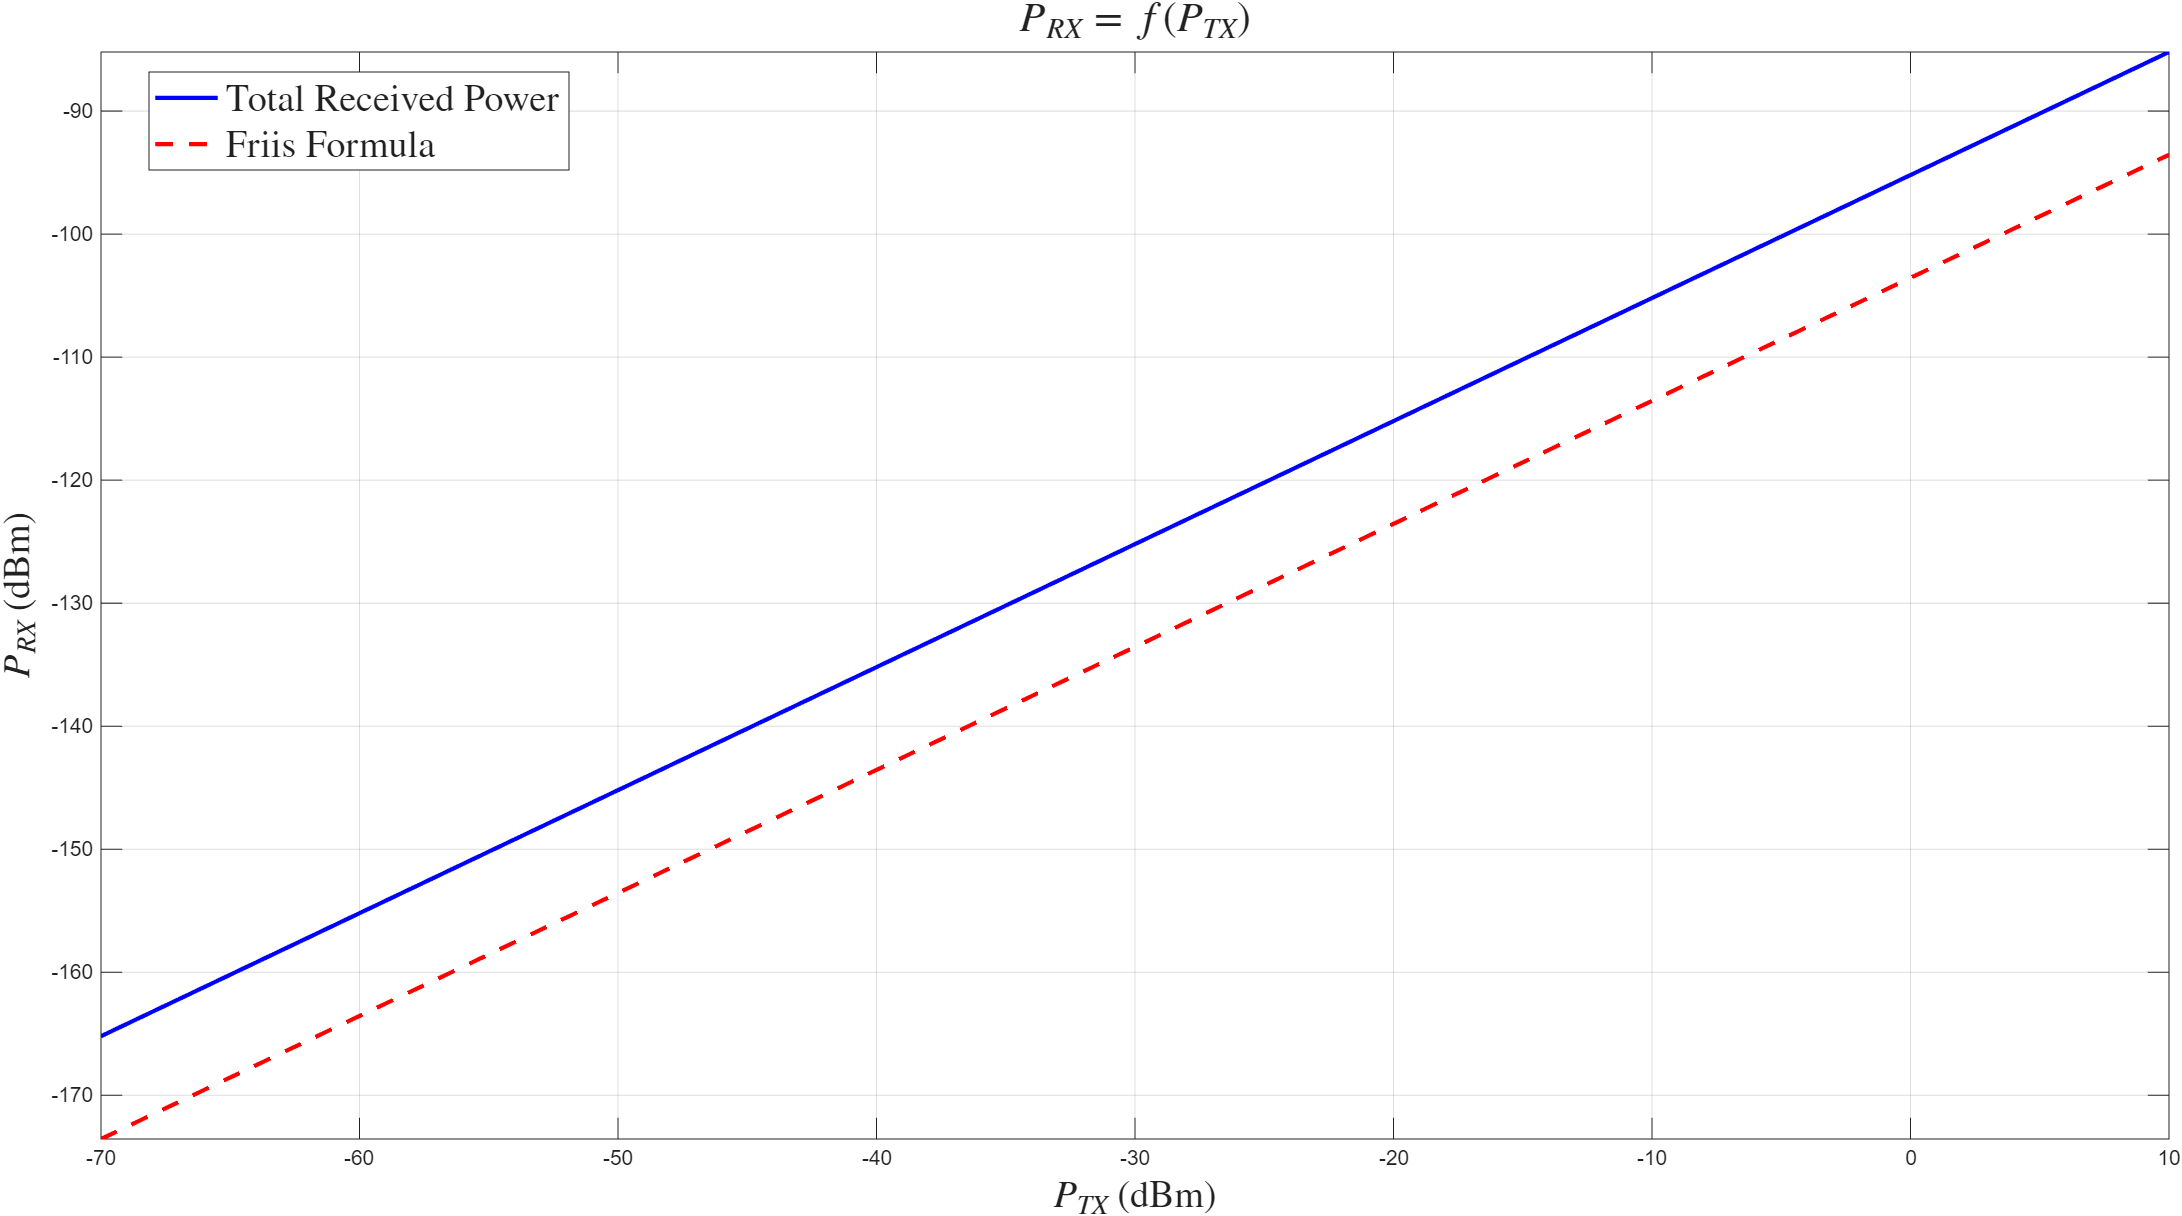
\includegraphics[width=1\linewidth]{content/4-images/PRX-vs-PTX}
	\caption{Received Power as a function of the Transmitted Power for a fixed channel ($d$ is constant and equal to $1km$). The number of reflections is $M=10$}
	\label{fig:prx-vs-ptx}
\end{figure}


This coherent summation results in fast fading for small distances and slow fading for very high distances between TX and RX. \\
Unlike the monotonic decrease of power with all distances predicted by the Friis formula, the full-channel received power will exhibit significant fluctuations as the distance $d$ changes at smaller distances. As seen in Figure \ref{fig:pRX_vs_friis}, for very high values of d, the models gets closer to the Friis formula, because the reflected rays will be drastically attenuated, compared to the LOS ray
\begin{itemize}
	\item \textbf{Constructive Interference:} At locations where the MPCs arrive largely in-phase, their amplitudes add up, resulting in a received power that can be significantly higher than the Friis prediction.
	\item \textbf{Destructive Interference:} At locations where some MPCs arrive out-of-phase, their amplitudes cancel each other out, leading to drops far below the Friis prediction.
\end{itemize}

\begin{figure}[h!]
	\centering
	% You should generate this plot using simulation tools (e.g., MATLAB, Python)
	% based on the derived equations for the 7 MPCs.
	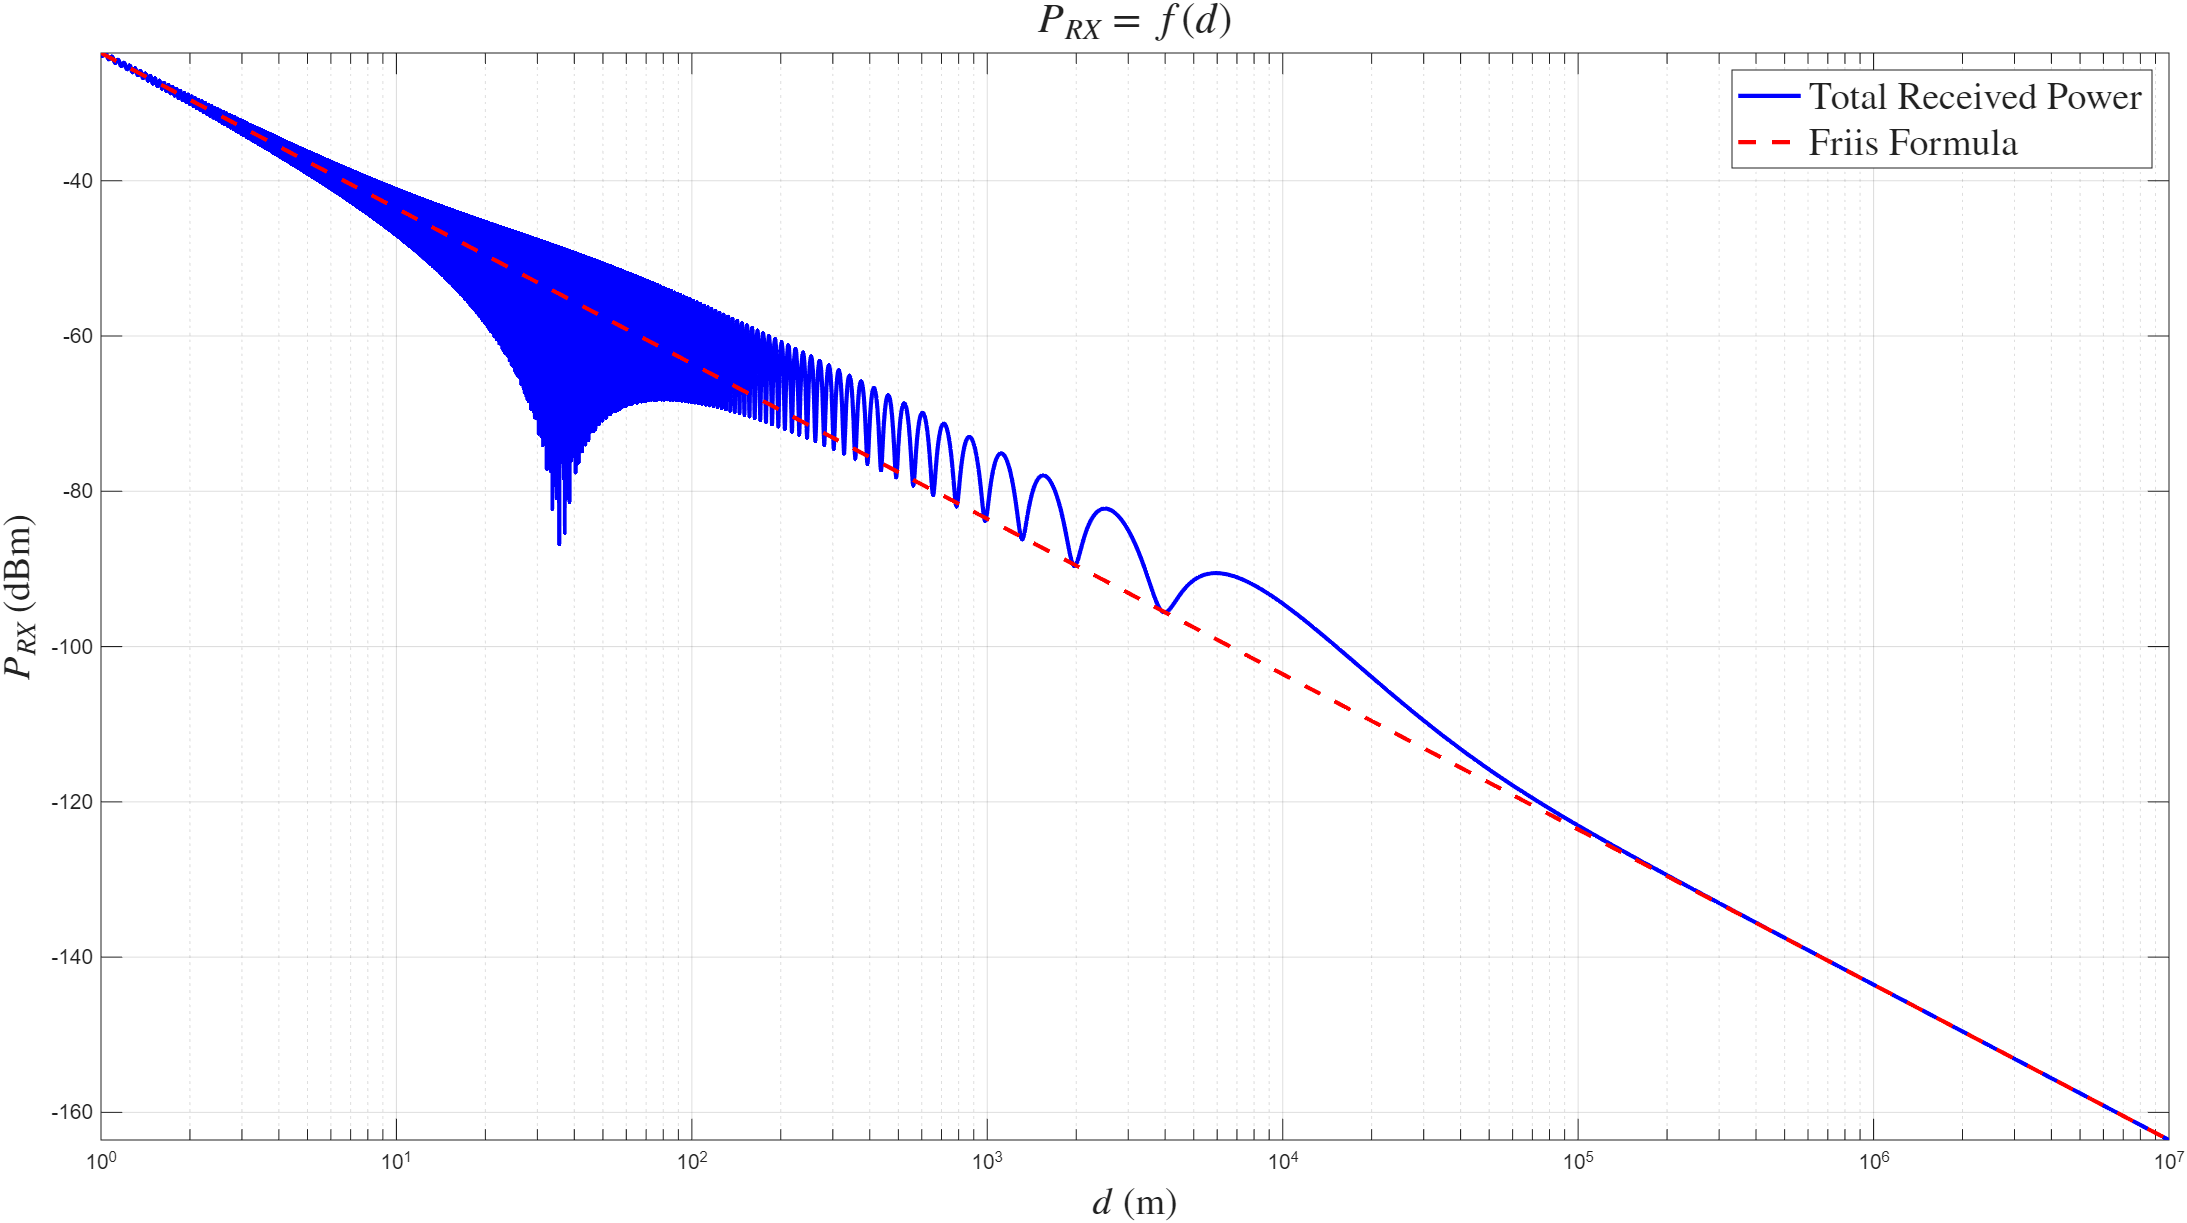
\includegraphics[width=\linewidth]{content/4-images/PRX-vs-Friis.png} % Placeholder ray
	\caption{Received power as a function of the separation distance between TX and RX in the Multipath Narrow band scenario for $M=1$ Reflection}
	\label{fig:pRX_vs_friis}
\end{figure}

\section{Rician factor}
The Rician factor $K$ is a parameter that quantifies the severity of fading in a channel. 
\begin{equation}
	K = \frac{|\alpha_{LOS}|^2}{\sum_{n=2}^{7} |\alpha_n|^2} = \frac{P_{LOS}}{P_{NLOS}}
\end{equation}
To evaluate this, we need to express $|\alpha_n|^2$ in terms of physical parameters. From the LOS analysis made earlier, we found that the received power for the direct ray is identical to the Friis formula:
\begin{equation}
	P_{LOS} = |\alpha_{LOS}|^2 P_{TX} = G_{TX} G_{RX} \left( \frac{\lambda}{4\pi d} \right)^2 P_{TX}
\end{equation}
This gives us the power gain for the LOS component ($d_1 = d$, $|\Gamma_1|^2=1$):
\begin{equation}
	|\alpha_{LOS}|^2 = G_{TX} G_{RX} \left( \frac{\lambda}{4\pi d} \right)^2
\end{equation}
For the $n$-th MPC that is not the LOS ray, and experiences reflections, the power is reduced by the cumulative reflection coefficient $\Gamma_n = \prod_{m=1}^{M}(\Gamma_{\perp, m}(\theta_{n}))$. The power gain for a reflected ray of total travel distance $d_n$ is therefore:
\begin{equation}
	|\alpha_n|^2 = G_{TX} G_{RX} \left( \frac{\lambda}{4\pi d_n} \right)^2 |\Gamma_n|^2
\end{equation}

Substituting these expressions for power gain into the K-factor equation:
\begin{equation}
	K = \frac{G_{TX} G_{RX} \left( \frac{\lambda}{4\pi d} \right)^2}{\sum_{n=2}^{7} G_{TX} G_{RX} \left( \frac{\lambda}{4\pi d_n} \right)^2 |\Gamma_n|^2}
\end{equation}
The common terms, including antenna gains and wavelength, cancel out, leaving a purely geometric relationship:
\begin{equation}
	K = \frac{\frac{1}{d^2}}{\sum_{n=2}^{7} \frac{|\Gamma_n|^2}{d_n^2}} \implies \boxed{K =\frac{1}{d^2 \sum_{n=2}^{7} \frac{|\Gamma_n|^2}{d_n^2}}}
\end{equation}
A high K-factor indicates that the channel is dominated by the LOS ray, and fading will be less severe leading to the Rician distribution. A low K-factor indicates that the NLOS rays are stronger relative to the LOS ray, leading to deep fades characteristic of Rayleigh distribution.

\begin{figure}
	\centering
	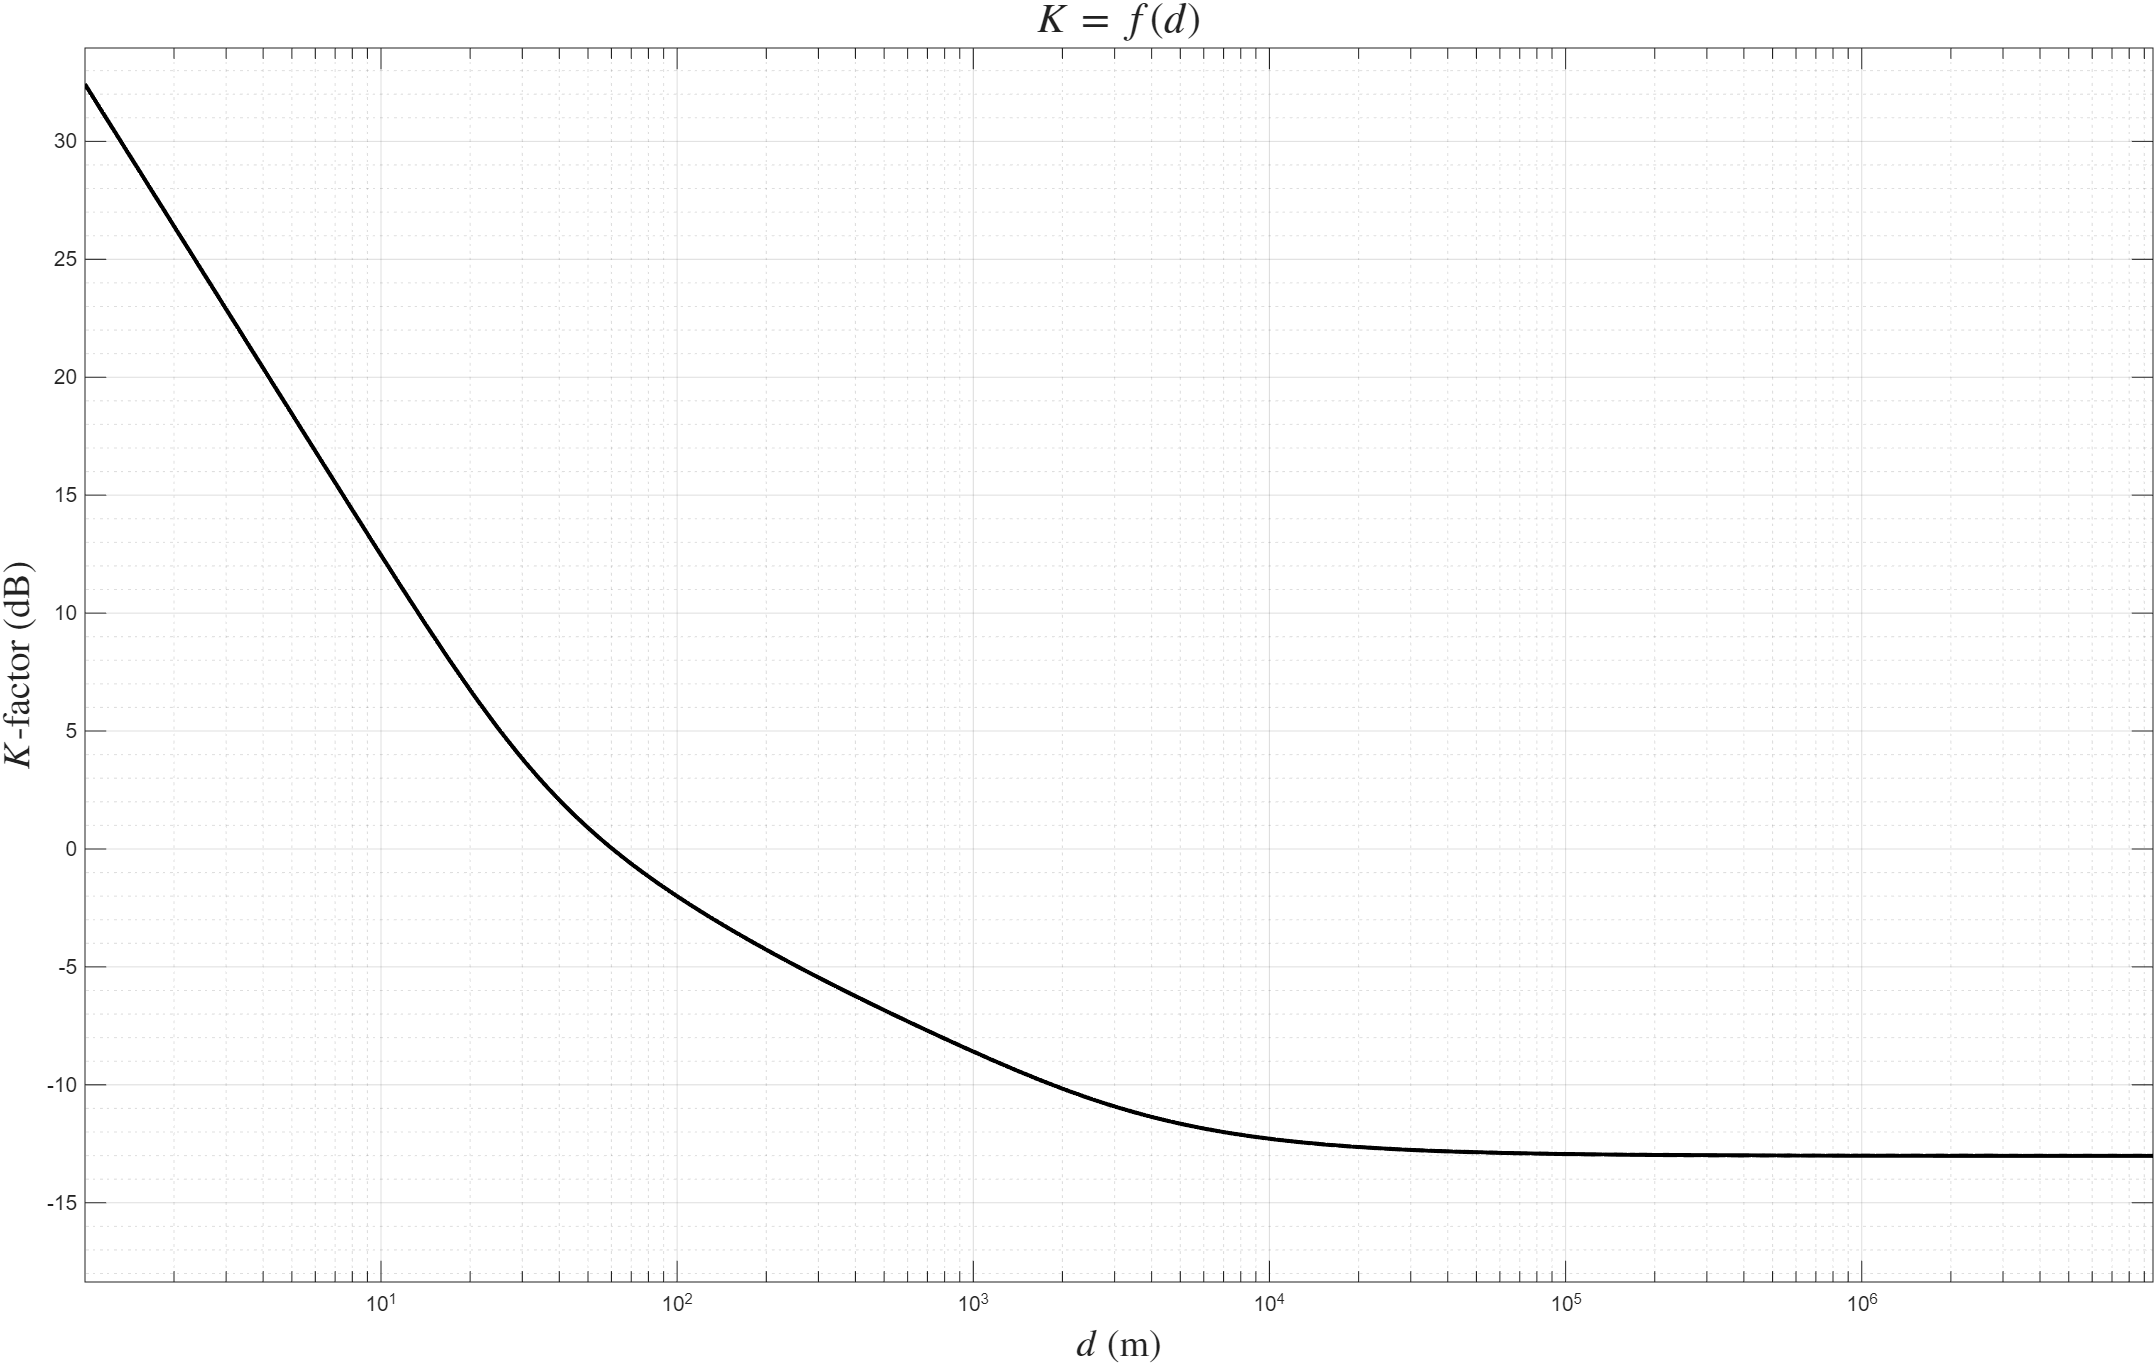
\includegraphics[width=\linewidth]{content/4-images/k-factor}
	\caption{K-factor as a function of the separation distance between TX and RX for $K=10$ reflections}
	\label{fig:k-factor}
\end{figure}




\section{Path Loss Model}
To analyze the large-scale path loss characteristics of the channel, the effects of small-scale fading, which arise from the rapid phase changes of the MPCs, must be averaged out. This is accomplished by computing the local average of the received power, $\langle P_{RX} \rangle$, in 5-meter segments. This spatial averaging smooths out the fast fluctuations, revealing the underlying distance-dependent trend.

The continuous-time definition of this local average at a distance $d$ is given by the integral:
\begin{equation}
	\langle P_{RX}(d) \rangle = \frac{1}{5m} \int_{d-2.5m}^{d+2.5m} P_{RX}(x) dx
\end{equation}
In the simulation, where the received power is sampled at discrete points, this integral is approximated by a discrete summation. This is implemented as a moving average filter, which mathematically corresponds to a discrete convolution. The instantaneous power signal, $P_{RX}[i]$, is convolved with a normalized rectangular kernel, $h[k]$, of length $N_{samp, local}$. This length corresponds to the number of samples within the 5m averaging window. The kernel is defined as:
\begin{equation}
	h[k] = 
	\begin{cases} 
		\frac{1}{N_{samp, local}} & \text{for } 0 \le k < N_{samp, local} \\ 
		0 & \text{otherwise} 
	\end{cases}
\end{equation}
This corresponds to a vector, $\mathbf{h}$, of $N_{samp, local}$ uniformly weighted coefficients:
\begin{equation}
	\mathbf{h} = \frac{1}{N_{samp, local}} \cdot
	\underbrace{\begin{bmatrix}
			{1, 1, \dots, 1}
	\end{bmatrix}}_{N_{samp, local} \text{ elements}}
\end{equation}
The resulting averaged power at sample $i$, which is the convolution $(P_{RX} * h)[i]$, is then given by:
\begin{equation}
	\langle P_{RX}[i] \rangle = \sum_{k=0}^{N_{samp, local}-1} P_{RX}[i-k] \cdot h[k] = \frac{1}{N_{samp, local}} \sum_{k=0}^{N_{samp, local}-1} P_{RX}[i-k]
\end{equation}

$N_{samp, local}$ is defined as:
\begin{equation}
	N_{samp} = \text{round}\left(\frac{\text{local window distance}}{\text{sampling distance}}\right)
\end{equation}






The path loss of the channel is defined as $L(d)$ such that:
\begin{align}
	\label{eq:loss}
	L_{data}(d) [dB] &= P_{TX} [dBm] - \langle P_{RX}(d) \rangle [dBm]\\
			  &= L_{0, data}(d) [dB] - 10 \log G_{TX} - 10 \log G_{RX} \label{eq:loss-3}
\end{align}
Where $L_0(d)$ represent the part of the path loss that does not depend on the antenna. Using Equation \eqref{eq:loss}, it can be expressed as:
\begin{align}
	L_{0, data}(d) [dB] &=  P_{TX} [dBm] + 10 \log G_{TX} + 10 \log G_{RX} - \langle P_{RX}(d) \rangle [dBm]
	\label{eq:loss-2}\\
				&= P_{TX} [dBm] + 2 \cdot G_{TX} [dBi] - \langle P_{RX}(d) \rangle [dBm]
\end{align}

It is empirically proven that in general the path loss model follows the canonical form:
\begin{align}
	L_{0}(d) [dB] &= L_0(d_0) + 10n \log\left(\frac{d}{d_0}\right)\\
				&= \underbrace{10n}_{slope} \log(d) + \underbrace{(L_0(d_0) - 10n \log(d_0))}_{intercept} \label{eq:lin-reg}
\end{align}


Where $d_0$ is a reference distance, and $n$ is the path loss exponent. This exponent describes how quickly the signal attenuates with distance on a large scale.

$n$ and $L_0(d_0)$ can be found by performing a linear regression. When $L_0(d)$ is found, it is simply replace in Equation \ref{eq:loss-3} to find $L(d)$












\section{Variability $\sigma_L$}
The variability, or shadowing standard deviation $\sigma_L$, quantifies the variation of the actual received power around the path loss model prediction. It is calculated as the standard deviation of the difference (in dB) between the local-area averaged power and the path loss model prediction.
\begin{equation}
	\sigma_L^2 = \text{Var} \left[ 10\log(\langle P_{RX} \rangle) - (P_{TX}[dBm] - L(d)[dB]) \right]
\end{equation}

\section{Fade Margin and Cell Range}
Assuming the power variations around the path loss model are log-normally distributed, we can determine the fade margin ($M$) required to achieve a certain communication reliability. The reliability is the probability that the received power is above the receiver sensitivity ($P_{sens} = -70$ dBm).
\begin{equation}
	\text{Pr}(P_{RX} > P_{sens}) = \text{Reliability}
\end{equation}
The fade margin is the extra power (in dB) needed to overcome fading. The maximum allowable path loss for a given reliability is $L_{max} = P_{TX}[dBm] - P_{sens}[dBm] - M$. The cell range is the distance $d$ at which the path loss $L(d)$ equals this maximum allowable path loss. We can calculate the required margin for 50\%, 95\%, and 99\% reliability and the corresponding cell ranges.

\section{Interpretation of Results}
The introduction of reflections from buildings fundamentally changes the channel behavior compared to the simple LOS case.
\begin{itemize}
	\item \textbf{Multiray Fading:} The total received power is no longer a monotonic function of distance. The vector sum of the MPCs creates an interference pattern, causing rapid and deep fluctuations in signal strength (fading) as the distance $d$ changes. This is a critical feature of real-world urban channels.
	\item \textbf{Rician K-factor:} The K-factor provides a quantitative measure of the channel's nature. For short distances $d$, the LOS ray is much stronger than the reflected rays, resulting in a high K-factor and a Rician-like distribution with moderate fading. As $d$ increases, the LOS power decreases, and the reflected rays become relatively more significant, lowering the K-factor and making the channel behave more like a Rayleigh fading channel.
	\item \textbf{path loss Exponent:} The path loss exponent $n$ derived from the averaged power will likely be greater than 2 (the free-space value). This is because the multiray environment tends to confine the energy, creating a "waveguide" effect that can alter the rate of power decay with distance.
	\item \textbf{Fade Margin and Reliability:} The variability $\sigma_L$ necessitates a fade margin to ensure reliable communication. A higher desired reliability (e.g., 99\% vs. 95\%) requires a larger fade margin, which in turn reduces the maximum communication range for the system. This highlights the trade-off between reliability and coverage in a fading channel.
\end{itemize}
